\begin{frame} \frametitle{\vspace*{0.5cm}Results: Evolution of the interface after 10 MPa trapezoidal wave}
  \begin{figure}
    \centering
    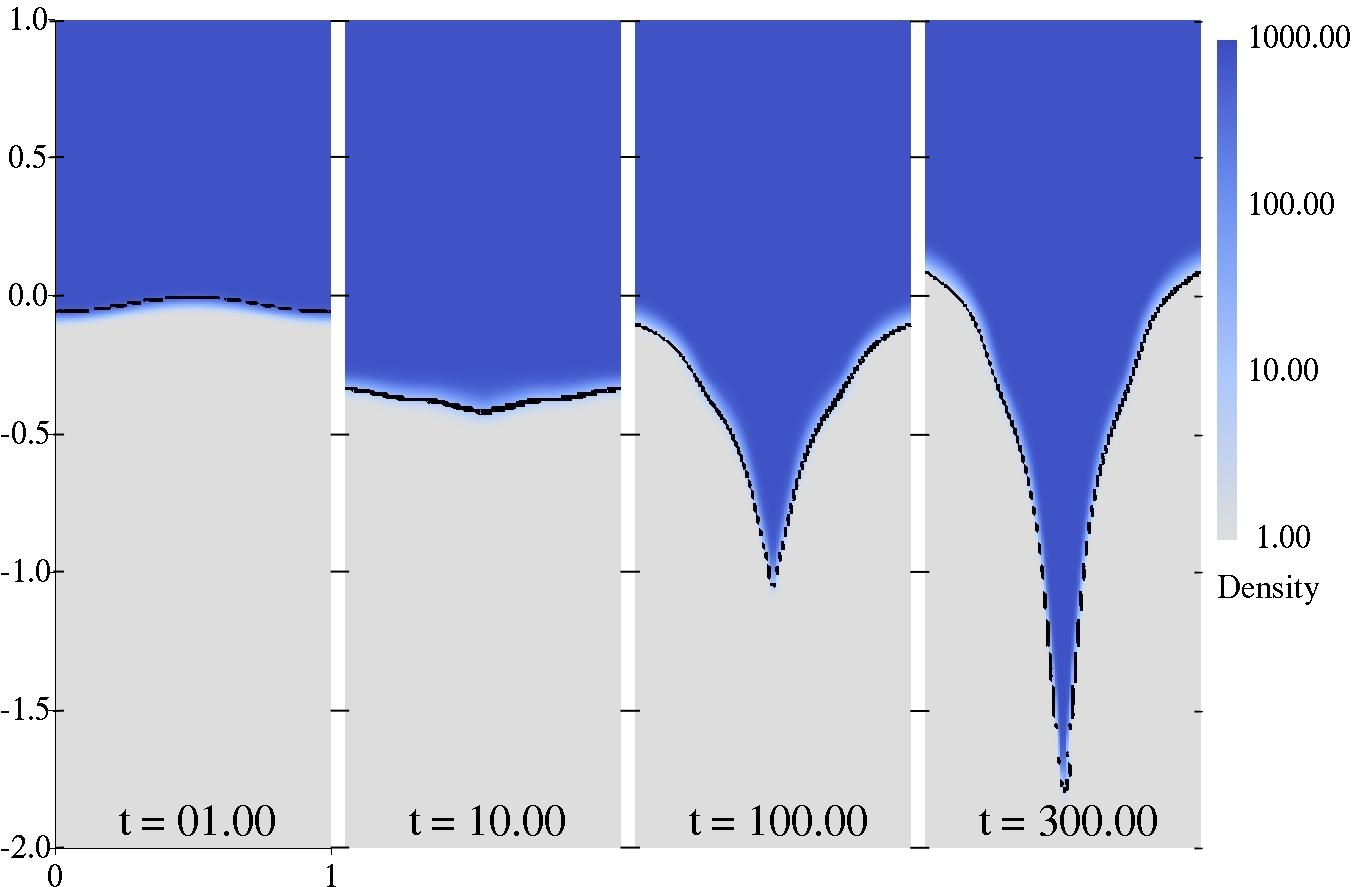
\includegraphics[width=0.85\textwidth]{../figs/lung_figs/snapshots_density_t1}
  \end{figure}
  {\small
    The interface perturbation evolves from a smooth sinusoid into a sharp point.
  }
  \note{
    \begin{enumerate}
    \item To illustrate qualitative behavior of the interface, density contours have been shown for the 10 MPa trapz wave case.
    \item The interface is initially smooth and looks sinusoidal even at $t=1$, when the compression has nearly passes.
    \item At $t=10$ the wave has passed, and the interface has inverted phase, or flipped direction and is no long sinusoidal.
    \item The interface perturbation continues to grow to a sharp point, long after the wave has passed.
    \item Note that time scales here are dimensionless and $t=300$ corresponds to about 100 microseconds
    \end{enumerate}
  }
\end{frame}
%%% Local Variables:
%%% mode: latex
%%% TeX-master: "../main"
%%% End:
